\documentclass{article}
\usepackage{amsmath}
\usepackage{amssymb}
\usepackage{graphicx}
\usepackage{siunitx}
\newcommand*\diff{\mathop{}\!\mathrm{d}}

\title{CS 244 Programming Assignment 2}
\author{Yutian Li\\ \texttt{yutian} \and Ryan Propper\\ \texttt{rpropper}}
\date{Team name: ``Occam's Router''}

\begin{document}
\maketitle

Link to our GitHub repo:  \texttt{https://github.com/hotpxl/occams-router}

\section*{Exercise A}

For each fixed window size $n$, ranging over the powers of 2 from 2 to 512, we ran the experiment three times. The best fixed window size we found is 16, achieving a throughput of 2.73 Mbits/s and 95th percentile signal delay of 229 ms (power score 11.92). Most of the times the points from a window size lie close to each other, indicating that the measurements are fairly repeatable. Also noteworthy is the convex shape of the plot: it represents the delay-throughput trade-off we face when choosing parameters. Bigger window sizes lead to higher throughput, but longer delay. The graph is shown below.

\begin{center}
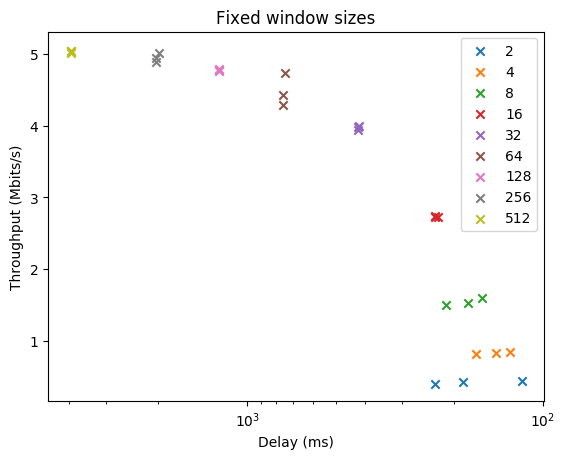
\includegraphics[width=0.9\textwidth]{images/exercise_a.png}
\end{center}

Clearly fixed window sizes are a poor choice for cellular networks that have high variability in both bandwidth and RTT. As seen in the plot above, small window sizes (such as $n = 2$ or $n = 4$) result in very little delay, but the link is under-utilized so throughput is quite poor. On the other hand, large window sizes saturate the link, pushing throughput near peak but also building up massive delays.

\section*{Exercise B}
The standard AIMD approach, as used by TCP, does not work very well. We chose an RTT of 100 ms as a threshold: an RTT greater than this is considered as a congestion signal, and will trigger a multiplicative decrease of window size. The goal is to stabilize RTT around 100 ms, where the minimum RTT of the link is 40 ms. We increase the window size by $\alpha=1$ if the RTT is less than this threshold, and multiply by $\beta=\frac{1}{2}$ if it exceeds this threshold.

As the results show, the average throughput is 2.70 Mbits/s and 95th percentile signal delay is 136 ms, achieving a power score of 19.85. Although it is definitely better than a fixed window size scheme, it still performs badly with highly unpredictable cellular networks. When the algorithm detects congestion on the link, it is already too late. Furthermore, the window size increases are generally too slow to achieve good throughput.

\section*{Exercise C}
We attempted this exercise using two watermarks. When the latency reaches low watermark, window is expanded, and when the latency hits high watermark, window is shrunk. Every time, the window is expanded or shrunk by one.

We tried all combinations of low watermarks from 50 to 90 in increments of 10 and high watermarks from 100 to 400 in increments of 50. The best result we have is when low watermarks is 50 and high watermark is 150. In this case, throughput is 4.35 Mbits/s and 95th percentile signal delay is 183 ms. The resulting power score is 23.83.

It is definitely better than previous experiments of fixed window size and AIMD scheme. But the problem is the window adjustment is too uniform and rigid, and is slow to adapt to sudden network changes.

All watermarks we attempted, and their results, are shown below.

\begin{center}
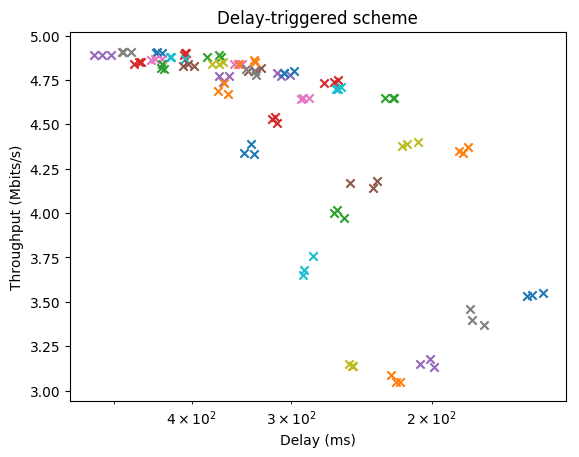
\includegraphics[width=0.9\textwidth]{images/exercise_c.png}
\end{center}

\section*{Exercise D}
Our overall approach is modeled on the BBR paper. We decided to implement a ``poor man's BBR'': constantly estimate the available bandwidth and keep the window size set to (or very close to) the BDP, bandwidth-delay product.

We first attempted some experiments with more aggressive AIMD, which didn't provide any useful results. We also attempted shrinking or growing the window size based on he ``slope'' of the measured bandwidth or RTT. For example, if the RTT was constant or growing slowly, we would continue to increase the window size; otherwise we would reduce it. This approach also did not work well.

Finally, motivated by the BBR paper, we settled on trying to estimate the available bandwidth periodically, and setting the window size equal to the estimated bandwidth-delay product. The algorithm, essentially, is:

\begin{enumerate}
    \item Periodically estimate the link's bandwidth, which we measure in packets per millisecond (ppms). We perform this calculation every \texttt{kInterval} milliseconds, on both packet sending and ACK receipt, by recording how many ACKs we received in that time. We maintain the most recent \texttt{kMaxEstimates} estimates in the \texttt{ppms\_} deque.
    \item When computing the window size, set it to an estimated bandwidth-delay product $B \cdot R$. Here $B$ is the estimated bandwidth; we take the average of the most recent \texttt{kMaxEstimates} samples. $R$ is a scaling factor, \texttt{kBwAggressiveness}, multiplied by the theoretical minimum RTT of the link; that is, $R = c \cdot \text{RTT}_{min}$. We estimate $\text{RTT}_{min}$ by observing all RTT samples and taking the lowest of all observed.
\end{enumerate}

As shown above, there are three primary parameters (which we have placed in \texttt{controller.hh}) that can be used to tune our algorithm:

\begin{enumerate}
    \item \texttt{kInterval}, approximately how frequently (in milliseconds) we perform a bandwidth estimate. We found \texttt{kInterval = 25} works well in practice.
    \item \texttt{kMaxEstimates}, how many recent bandwidth (packet/ms) estimates to keep We found \texttt{kMaxEstimates = 5} works well in practice, and it seemed reasonable to use several estimates (but not too many) to smooth the bandwidth estimates.
    \item \texttt{kBwAggressiveness}, the factor used to scale our observed $RTT_{min}$ when computing the window size as the BDP. We found \texttt{kBwAggressiveness} values between 1.5 and 1.75 seemed to work well in practice; higher values attempt to gain more bandwidth at a cost of higher average latency.
\end{enumerate}

For example, the graph below shows the power scores we obtained when setting \texttt{kBwAggressiveness = 1.75} and varying \texttt{kMaxEstimates}:

\begin{center}
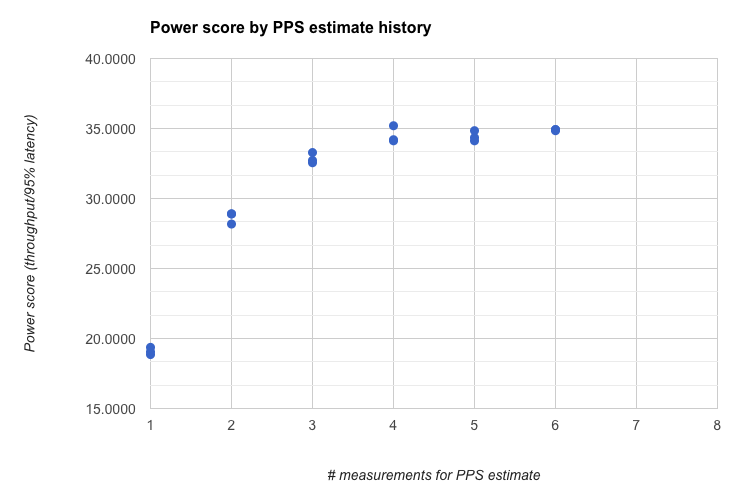
\includegraphics[width=1.0\textwidth]{images/exercise_d_power_score.png}
\end{center}

And this graph shows the effect of adjusting \texttt{kBwAggressiveness} while using a fixed \texttt{kMaxEstimates = 5}:

\begin{center}
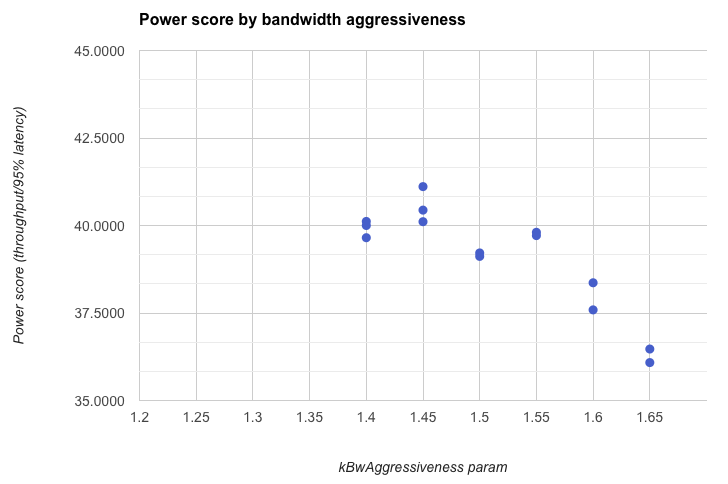
\includegraphics[width=1.0\textwidth]{images/exercise_d_bw_aggressiveness.png}
\end{center}

Overall we found this approach to be reasonably effective with the provided sample trace. On a Google Compute Engine virtual machine, we obtained about 4 Mbits/s average throughput and 95th percentile signal delay around 100 to 105 ms. The highest power score we achieved with this algorithm across all of our tests is 41.11, which seems competitive with Sprout.

\end{document}
